\documentclass[12pt]{beamer}

\usepackage[brazil]{babel}
\usepackage[utf8]{inputenc}
\usepackage[T1]{fontenc}
\usepackage{animate}
\usepackage{amsbsy}
\usepackage{amsfonts}
\usepackage{amsmath}
\usepackage{amssymb}
\usepackage{amsthm}
\setbeamertemplate{theorems}[numbered] % to number
\usepackage[toc,page,title,titletoc]{appendix}
\usepackage{dsfont}
\usepackage{esvect}
\usepackage[labelfont=bf]{caption}
%\usepackage{subcaption}
\usepackage{float}
\usepackage[Glenn]{fncychap}%Sonny %Conny %Lenny %Glenn %Renje %Bjarne %Bjornstrup
\usepackage{graphicx}
\usepackage{subfig}
\usepackage{indentfirst}%Para indentar os paragrafos automáticamente
\usepackage{lipsum}
\usepackage{longtable}
\usepackage{mathtools}
\usepackage{listings}%Inserir codigo do R no latex
\usepackage{multirow}
\usepackage{multicol}
\usepackage{csquotes}
\usepackage[maxcitenames=2,terseinits=true,natbib=true, style=authoryear, maxbibnames=99]{biblatex}
\addbibresource{../Referencias/Referencias.bib}
\usepackage[figuresright]{rotating}
\usepackage{spalign}
\usepackage{pgfplots}
\pgfplotsset{compat=1.17}
\usepackage{tikz}
\usepackage{fontawesome}
\usepackage{color, colortbl}
\usepackage{url}
\usepackage{cancel}
\usepackage{accents}
\usepackage{bm}
\usepackage{ragged2e}%para justificar o texto dentro de algum ambiente
\definecolor{Gray}{gray}{0.9}
\definecolor{LightCyan}{rgb}{0.88,1,1}


\usepackage[all]{xy}
\usepackage{hyperref,bookmark}
\hypersetup{
  colorlinks=true,
  linkcolor=blue,
  citecolor=red,
  filecolor=blue,
  urlcolor=blue,
}

\usetheme{Madrid}
\usecolortheme[RGB={193,0,0}]{structure}

%\setbeamertemplate{footline}[frame number]
%\setbeamertemplate{footline}[text line]{%
%  \parbox{\linewidth}{\vspace*{-8pt}\hfill\date{}\hfill\insertshortauthor\hfill\insertpagenumber}}
\beamertemplatenavigationsymbolsempty
\renewcommand{\vec}[1]{\mbox{\boldmath$#1$}}
\newtheorem{Teorema}{Teorema}
\newtheorem{Proposicao}{Proposição}
\newtheorem{definicao}{Definição}
\newtheorem{Corolario}{Corolário}
\newtheorem{Demonstracao}{Demonstração}
\newcommand{\bx}{\ensuremath{\bar{x}}}
\newcommand{\Ho}{\ensuremath{H_{0}}}
\newcommand{\Hi}{\ensuremath{H_{1}}}
\newcommand{\at}[2][]{#1|_{#2}}
\newcommand\xuparrow[1][2ex]{%
   \mathrel{\rotatebox{-90}{$\xleftarrow{\rule{#1}{0pt}}$}}
}
\apptocmd{\frame}{}{\justifying}{} % Allow optional arguments after frame.

\makeatletter
\setbeamertemplate{footline}
{
  \leavevmode%
  \hbox{%
  \begin{beamercolorbox}[wd=.3\paperwidth,ht=2.25ex,dp=1ex,center]{author in head/foot}%
    \usebeamerfont{author in head/foot}\mytext
  \end{beamercolorbox}%
  \begin{beamercolorbox}[wd=.3\paperwidth,ht=2.25ex,dp=1ex,center]{title in head/foot}%
    \usebeamerfont{title in head/foot}\mytextt
  \end{beamercolorbox}%
  \begin{beamercolorbox}[wd=.35\paperwidth,ht=2.25ex,dp=1ex,right]{site in head/foot}%
    \usebeamerfont{site in head/foot}\mytexttt\hspace*{2em}
    \insertframenumber{} / \inserttotalframenumber\hspace*{2ex} 
  \end{beamercolorbox}}%
  \vskip0pt%
}
\makeatother

\providecommand{\arcsin}{} \renewcommand{\arcsin}{\hspace{2pt}\textrm{arcsen}}
\providecommand{\sin}{} \renewcommand{\sin}{\hspace{2pt}\textrm{sen}}
\newcommand{\N}{\rm I\!N}
\newcommand{\I}{\rm I\!I}
\newcommand{\R}{\rm I\!R}
\newcommand{\Sim}{\overset{\text{iid}}{\sim}}
\newcommand{\Lim}{{\displaystyle \lim_{n\to\infty}}}
\newcommand{\LimInf}{{\displaystyle \liminf_{n\to\infty}}}
\newcommand{\rightLim}{\xrightarrow[n\rightarrow\infty]{}}
\newcommand{\Sumi}{{\displaystyle \sum_{i=1}^{n}}}
\newcommand{\Int}{{\displaystyle \int_{-\infty}^{+\infty}}}
\newcommand{\ConvD}{\overset{D}{\rightarrow}}
\newcommand{\ConvP}{\overset{P}{\rightarrow}}
\newcommand{\Prodi}{{\displaystyle \prod_{i=1}^{n}}}
\newcommand{\SetaUP}[2]{\underset{\mathclap{\substack{\xuparrow[30pt] \\ #1}}}{#2}}
%\newcommand{\SetaInclinada}[2]{\underset{\mathclap{\substack{\rotatebox{135}{\xuparrow[30pt] \\ #1}}}}{#2}}
\newcommand{\Home}{\begin{tikzpicture}
\node[scale=2] at (3,4) {\text{Para}~\faHome};
\end{tikzpicture}}
\newcommand{\vecX}{\boldsymbol{X}}
\newcommand{\Implica}[1]{\xRightarrow{#1}}
\newcommand{\SeSe}{\iff}
\newcommand{\EscoreA}{\dfrac{\partial}{\partial\theta}\log{f(x,\theta)}}
\newcommand{\EscoreB}{\dfrac{\partial^{2}}{\partial\theta^{2}}\log{f(x,\theta)}}
\newcommand{\cqd}{\text{cqd}~\blacksquare}
\newcommand{\seqX}{$X_{1},\ldots,X_{n}$}
\newcommand{\seqY}{$Y_{1},\ldots,Y_{n}$}
\newcommand{\tend}[1]{\hbox{\oalign{$\bm{#1}$\crcr\hidewidth$\scriptscriptstyle\bm{\sim}$\hidewidth}}}

%\newtheorem{Teorema}{Teorema}
%\newtheorem{Proposicao}{Proposição}
%\newtheorem{Definicao}{Definição}
%\newtheorem{Corolario}{Corolário}
%\newtheorem{Demonstracao}{Demonstração}

\titlegraphic{\hspace*{8cm}\href{https://fsbmat-ufv.github.io/}{
\includegraphics[width=2cm]{figs/mylogo.png}}
}

%Continuar a numeracao em slides diferentes
\newcounter{saveenumi}
\newcommand{\seti}{\setcounter{saveenumi}{\value{enumi}}}
\newcommand{\conti}{\setcounter{enumi}{\value{saveenumi}}}

\resetcounteronoverlays{saveenumi}

% Layout da pagina
\hypersetup{pdfpagelayout=SinglePage}

%Para o \pause funcionar dentro do ambiente align
\makeatletter
\let\save@measuring@true\measuring@true
\def\measuring@true{%
  \save@measuring@true
  \def\beamer@sortzero##1{\beamer@ifnextcharospec{\beamer@sortzeroread{##1}}{}}%
  \def\beamer@sortzeroread##1<##2>{}%
  \def\beamer@finalnospec{}%
}
\makeatother


\title{Inferência Estatística II}
\author{Prof. Fernando de Souza Bastos\texorpdfstring{\\ fernando.bastos@ufv.br}{}}
\institute{Departamento de Estatística\texorpdfstring{\\ Programa de Pós-Graduação em Estatística Aplicada e Biometria}\texorpdfstring{\\ Universidade Federal de Viçosa}{}\texorpdfstring{\\ Campus UFV - Viçosa}{}}
\date{}
\newcommand\mytext{Aula 7}
\newcommand\mytextt{Fernando de Souza Bastos}
\newcommand\mytexttt{\url{https://est711.github.io/}}


\begin{document}
%\SweaveOpts{concordance=TRUE}

\frame{\titlepage}

\begin{frame}{}
\frametitle{\bf Sumário}
\tableofcontents
\end{frame}

\section{Propriedades dos Estimadores}
\begin{frame}{Introdução}
\frametitle{}
\begin{block}{}
\justifying
Propriedades dos estimadores são uma questão fundamental na inferência estatística, pois elas determinam a qualidade e a confiabilidade das estimativas obtidas a partir dos dados amostrais. Um estimador é uma função dos dados amostrais que é usada para estimar um parâmetro desconhecido da população subjacente. As propriedades dos estimadores descrevem como eles se comportam em diferentes situações, como a amostra aumentando de tamanho ou a população apresentando diferentes características. As principais propriedades dos estimadores incluem viés, consistência, eficiência e robustez. O conhecimento dessas propriedades é essencial para avaliar a qualidade de um estimador e para tomar decisões informadas com base nas estimativas obtidas a partir dos dados. 
\end{block}
\end{frame}

\subsection{Viés}
\begin{frame}{}
\begin{block}{}
\justifying
Ao criar um estimador de parâmetros, uma questão fundamental é saber se o estimador difere ou não do parâmetro de maneira sistemática.
\begin{definicao}\label{def1}
\justifying
Seja $X=(X_{1},X_{2},...,X_{n})$ uma amostra aleatória de uma variável aleatória $X$ com função de densidade $f(x;\theta)$, $\theta \in \Omega$. Seja $T = T(X_1, X_2, \dots, X_n)$ um Estimador de $\theta$. O \textbf{Viés} ($b(\theta)$) é a média da diferença de $T(X)-\theta,$ isto é, $$b(T(X))=E(T(X))-\theta$$.
\end{definicao}
\end{block}
\end{frame}

\begin{frame}{}
%\begin{block}{}
%\justifying
\begin{definicao}\label{def2}
\justifying
Seja $X=(X_{1},X_{2},...,X_{n})$ uma amostra aleatória de uma variável aleatória $X$ com função de densidade $f(x;\theta)$, $\theta \in \Omega$. Seja $T = T(X_1, X_2, \dots, X_n)$ um Estimador de $\theta$. Dizemos que $T$ é um estimador não viesado de $\theta$ se $E(T)=\theta,$ ou seja, se $$b(T(X))=0.$$
\end{definicao}
\pause
\begin{definicao}\label{def3}
\justifying
Se ${\displaystyle \lim_{n\rightarrow \infty}b(T(X))=0}$ para
todo $\theta \in \Theta$, dizemos que o estimador $T(X)$ é assintoticamente não viciado para $\theta$.
\end{definicao}
%\end{block}
\end{frame}

\begin{frame}{Exemplos 1}
\begin{block}{}
\begin{enumerate}
\justifying
    \item \textbf{Média amostral}: A média amostral é um estimador não viesado da média populacional. Isso significa que, em média, a média amostral estima corretamente a média populacional, sem inclinação para superestimá-la ou subestimá-la.

    \item \textbf{Variância amostral}: A variância amostral é um estimador não viesado da variância populacional. Isso significa que, em média, a variância amostral estima corretamente a variância populacional, sem inclinação para superestimá-la ou subestimá-la.

    \item \textbf{Estimador de máxima verossimilhança}: O estimador de máxima verossimilhança é um estimador não viesado que utiliza a função de verossimilhança para encontrar o valor mais provável do parâmetro populacional. Ele é amplamente utilizado em estatística inferencial para estimar parâmetros de distribuições populacionais.
\seti
\end{enumerate}
\end{block}
\end{frame}

\begin{frame}{Exemplos 2}
\begin{block}{}
\begin{enumerate}
 \conti
 \justifying
    \item \textbf{Mediana amostral}: A mediana amostral é um estimador não viesado da mediana populacional. Ao contrário da média, que pode ser influenciada por valores extremos, a mediana é mais robusta a essas observações e fornece uma medida mais representativa do centro da distribuição.

    \item \textbf{Estimador por momentos}: O estimador por momentos é um estimador não viesado que utiliza momentos da amostra para estimar parâmetros populacionais. Ele é uma abordagem simples e amplamente utilizada para estimar média, variância e outros momentos de uma distribuição populacional.

    \item \textbf{Desvio padrão amostral}: O desvio padrão amostral é um estimador viesado da variância populacional. Ele tende a subestimar a variância populacional, especialmente em amostras pequenas.
    \seti
\end{enumerate}
\end{block}
\end{frame}

\begin{frame}{Exemplos 3}
\begin{block}{}
\begin{enumerate}
 \conti
 \justifying
    \item \textbf{Média amostral truncada}: Este é um estimador de uma média populacional que é obtido a partir de uma amostra, mas em que alguns valores extremos são removidos antes de se calcular a média amostral. Se a amostra não for representativa da população, a média amostral truncada pode ser um estimador viesado.

    \item \textbf{Máximo da amostra}: O máximo da amostra é um estimador da ordem estatística mais alta da população. No entanto, se a amostra não for grande o suficiente, o máximo da amostra pode ser um estimador viesado.

    \item \textbf{Variância amostral não-corrigida}: A variância amostral é um estimador da variância populacional, mas se não for corrigida, isto é, dividida pelo tamanho da amostra menos 1, ela pode ser um estimador viesado.
\end{enumerate}
\end{block}
\end{frame}

\begin{frame}{Exemplo 4}
\begin{block}{}
\justifying
Suponha que a função densidade de probabilidade de uma amostra aleatória $X=(X_{1},X_{2},...,X_{n})$ seja $\Gamma(1,\theta),$ isto é, $f(x)=\theta^{-1}\exp{(\frac{-x}{\theta})},$ com suporte $0<x<\infty.$ Nesse caso, a distribuição gamma é também chamada de distribuição exponencial. O $\log{}$ da função de verossimilhança é dado por:
\begin{align*}
    \ell(\theta)=\log{{\displaystyle \prod_{i=1}^{n}}\dfrac{1}{\theta}e^{-x_{i}/\theta}}=-n\log{\theta}-\theta^{-1}{\displaystyle \sum_{i=1}^{n}x_{i}}
\end{align*}
A primeira derivada parcial do log-verossimilhança com respeito a $\theta$ é:
\begin{align*}
    \dfrac{\partial \ell(\theta)}{\partial \theta}=-n\theta^{-1}+\theta^{-2}{\displaystyle \sum_{i=1}^{n}x_{i}}
\end{align*}
\end{block}
\end{frame}

\begin{frame}{Continuação do Exemplo 4}
\begin{block}{}
\justifying
Definindo esta derivada parcial como $0$ e resolvendo para $\theta$, obtemos a solução $\Bar{x}$. Há apenas um valor crítico e, além disso, a segunda derivada parcial do logaritmo da verossimilhança avaliada em $\Bar{x}$ é estritamente negativa, o que confirma que ela fornece um máximo. Portanto, para este exemplo, a estatística $\hat{\theta} = \Bar{X}$ é a estimativa de máxima verossimilhança (MLE) de $\theta$. Como $E(X) = \theta$, temos que $E(\Bar{X}) = \theta$ e, portanto, $\hat{\theta}$ é um estimador não enviesado de $\theta$.
\end{block}
\end{frame}

\begin{frame}{Exemplo 5}
\begin{block}{}
\justifying
Seja $X=(X_{1},X_{2},...,X_{n})$ ensaios de Bernoulli com parâmetro de sucesso $p$, definimos o estimador para $p$ como sendo $d(X) = \Bar{X}$, a média amostral. Então,
\begin{align*}
    E_{p}(\Bar{X})&=\dfrac{1}{n}(E(X_{1})+\cdots+E(X_{n}))\\
    &=\dfrac{1}{n}(p+\cdots+p)=p
\end{align*}
Assim, $\Bar{X}$ é um estimador não viesado para $p.$ Neste caso, geralmente escrevemos $\hat{p}$ em vez de $\Bar{X}$, para representar a média amostral. 
\end{block}
\end{frame}

\begin{frame}{Continuação do Exemplo 5}
\begin{block}{}
\justifying
Podemos usar o fato de que, para variáveis aleatórias independentes, a variância da soma é a soma das variâncias, assim:
\begin{equation*}
Var(\hat{p}) = Var\left(\frac{1}{n}\sum_{i=1}^{n} X_i\right) = \frac{1}{n^2}\sum_{i=1}^{n} Var(X_i) = \frac{p(1-p)}{n}
\end{equation*}
\end{block}
\end{frame}

\begin{frame}{Exemplo 6}
\vspace{-0.5cm}
\begin{block}{}
\justifying
Se $X_1, \ldots, X_n$ formarem uma amostra aleatória simples com média finita e desconhecida $\mu$, então $\overline{X}$ é um estimador não enviesado de $\mu$. Se os $X_i$ possuem variância $\sigma^2$, então:
\begin{equation*}
Var(\overline{X}) = \frac{\sigma^2}{n}
\end{equation*}
\end{block}
\end{frame}

\begin{frame}{Continuação do Exemplo 6}
\begin{block}{}
\justifying
Com relação à variância amostral, temos
\begin{align*}
E[\hat{\sigma}^2] &= \frac{1}{n} E\left[\sum_{i=1}^n (X_i - \overline{X})^2\right] = \frac{1}{n} \sum_{i=1}^n E[(X_i - \overline{X})^2] \\
&= \frac{1}{n} \sum_{i=1}^n E\left[\left[(X_i - \mu) - (\overline{X} - \mu)\right]^2\right]=\dfrac{(n-1)}{n}\sigma^{2}
\end{align*}
Portanto, $\hat{\sigma}^2$ é viciado para $\sigma^2$, mas é assintoticamente não viciado, ou seja, à medida que o tamanho da amostra aumenta, o viés diminui.
\end{block}
\end{frame}

\subsection{Variância de um Estimador}
\begin{frame}{Variância de um Estimador}
\begin{block}{}
\justifying
É desejável que os estimadores de um determinado parâmetro da população possuam um valor de variância que seja o mínimo possível, isso porque uma variância baixa significa uma precisão maior da estimativa do que uma variância alta.

Podemos observar na Figura (Colocar Figura) que o histograma das médias aritméticas possui uma variabilidade menor do que o histograma dos primeiros valores das amostras. Além disso, ao aumentarmos o tamanho de cada amostra a variabilidade da média aritmética da amostra vai diminuindo, enquanto que a variabilidade do primeiro valor da amostra não diminui à medida que o tamanho da amostra aumenta.

Pode-se mostrar que a média aritmética da amostra é o estimador de menor variância entre todos os estimadores lineares da média de uma população. \textbf{O erro-padrão de um estimador é a raiz quadrada
da variância do estimador.}
\end{block}
\end{frame}

\subsection{Erro Quadrático Médio}
\begin{frame}{Erro Quadrático Médio}
\begin{block}{}
\justifying
Podemos avaliar a qualidade de um estimador calculando seu erro quadrático médio, definido por:

\begin{equation}\label{EQM1}
E[(T(X) - \theta)^2]
\end{equation}

Estimadores com erro quadrático médio menor são geralmente preferidos em relação a aqueles com erro quadrático médio maior. 
\end{block}
\end{frame}

\begin{frame}{}
\begin{block}{}
\justifying
Se escrevermos $Y = T(X) - \theta$ em (\ref{EQM1}) e lembrarmos que a variância é dada por $\text{Var}(Y) = E(Y^2) - (E(Y))^2$, então:

\begin{align*}
E(Y) &= E(T(X) - \theta)\\ 
&= E(T(X)) - \theta\\ 
&= b(T(X))
\end{align*}
e,
\begin{align*}
\text{Var}(Y) &= \text{Var}(T(X))
\end{align*}
Dessa forma, o erro quadrático médio é dado por:

\begin{align*}
E[(T(X) - \theta)^2] = E(Y^2) &= \text{Var}(Y) + (E(Y))^{2}\\
&=\text{Var}(T(X)) + b^2 (T(X))
\end{align*}
\end{block}
\end{frame}

\begin{frame}{}
\begin{block}{}
\justifying
Assim, a representação do erro quadrático médio como igual à variância do estimador mais o quadrado do viés é chamada de decomposição viés-variância. O erro quadrático médio pode ser considerado como uma medida da precisão de um estimador. Se a variância for pequena, podemos dizer que o estimador é preciso. Ele ainda pode não ser muito preciso se o viés for grande. Observem que:
\begin{itemize}
    \item O erro quadrático médio para um estimador não viciado é a sua variância.\pause
    \item O viés sempre aumenta o erro quadrático médio.
\end{itemize}

\end{block}
\end{frame}

\begin{frame}{}
\begin{block}{}
\justifying
O erro quadrático médio é comumente empregado na comparação de estimadores. Dizemos que o estimador $\hat{\theta}_1$ é melhor que o estimador $\hat{\theta}_2$ se

\begin{equation}
EQM[\hat{\theta}_1] \leq EQM[\hat{\theta}_2],
\end{equation}

para todo $\theta$, com $\leq$ substituído por $<$ pelo menos para um valor de $\theta$. Nesse caso, o estimador $\hat{\theta}_2$ é dito ser inadmissível. Se existir um estimador $\hat{\theta}^{*}$ tal que para todo estimador $\hat{\theta}$ de $\theta$ com $\hat{\theta} \neq \hat{\theta}^{*}$

\begin{equation}\label{EQMOtimo}
EQM[\hat{\theta}^{*}] \leq EQM[\hat{\theta}],
\end{equation}

para todo $\theta$ com $\leq$ substituído por $<$ para pelo menos um $\theta$, então $\hat{\theta}^{*}$ é dito ser ótimo para $\theta$. 
\end{block}
\end{frame}

\begin{frame}{}
\begin{block}{}
\justifying
Notemos que, se em (\ref{EQMOtimo}) os estimadores são não viciados, então $\hat{\theta}^{*}$ é dito ser o estimador não viciado de variância uniformemente mínima, se

\begin{equation}
Var[\hat{\theta}^{*}] \leq Var[\hat{\theta}],
\end{equation}

para todo $\theta$, com $\leq$ substituído por $<$ para pelo menos um $\theta$.
\end{block}
\end{frame}

\begin{frame}{Exemplo 1}
\begin{block}{}
\justifying
Sejam $X_1, X_2, X_3$ uma amostra aleatória da variável aleatória $X$ com $E[X] = \theta$ e $\mathrm{Var}[X] = 1$. Consideremos os estimadores 
\begin{align*}
    \hat{\theta}_1 = \Bar{X} = \frac{X_1 + X_2 + X_3}{3}~\textrm{e}~\hat{\theta}_2 = \frac{1}{2}X_1 + \frac{1}{4}X_2 + \frac{1}{4}X_3.
\end{align*}
\end{block}
\end{frame}

\begin{frame}{Continuação do Exemplo 1}
\begin{block}{}
\justifying
Temos que,
\begin{align*}
E[\hat{\theta}_1] &= \theta \quad \text{e} \quad Var[\hat{\theta}_1] = \frac{1}{3}\\
E[\hat{\theta}_2] &= \theta \quad \text{e} \quad Var[\hat{\theta}_2] = \frac{6}{16}
\end{align*}

Como ambos $\hat{\theta}_1$ e $\hat{\theta}_2$ são não viesados, segue que $\Bar{X}$ é um estimador melhor que $\hat{\theta}_2$, pois $Var[\Bar{X}] < Var[\hat{\theta}_2]$ para todo $\theta$.
\end{block}
\end{frame}

\begin{frame}{Exemplo 2}
\begin{block}{}
\justifying
Sejam $X_1, \ldots, X_n$ uma amostra aleatória da variável aleatória $X \sim N(\mu, \sigma^2)$. Conforme visto anteriormente, $\hat{\sigma}^2=\dfrac{1}{n} {\displaystyle \sum_{i=1}^{n}(X_i - \overline{X})^2}$ é um estimador viciado para $\sigma^2$. Sabe-se 
$$S^2 = \dfrac{n-1}{n}\sigma^2 = \dfrac{1}{n-1} \sum_{i=1}^{n} (X_i - \overline{X})^2$$
é um estimador não viciado para $\sigma^2$. Por outro lado, temos que

\begin{align*}
EQM[S^2] &= Var[S^2] = \frac{2\sigma^4}{n - 1}, \
EQM[\hat{\sigma}^2] &= \frac{2\sigma^4}{n - 1} \left( 1 - \frac{3n - 1}{2n^2} \right).
\end{align*}
\end{block}
\end{frame}

\begin{frame}{Continuação do Exemplo 2}
\begin{block}{}
\justifying
Notemos que $\hat{\sigma}^2$, apesar de viciado, apresenta um EQM menor que o EQM do estimador $S^2$.
\end{block}
\end{frame}

\begin{frame}{Exemplo 3}
\begin{block}{}
\justifying
Sejam $X_1, \ldots, X_n$ uma amostra aleatória de tamanho $n$ da variável aleatória $X$, com distribuição de Bernoulli com parâmetro $\theta$, ou seja, $Binomial(1, \theta)$. Conforme visto no modelo binomial, $Y = X_1 + \ldots + X_n$ tem distribuição binomial $Binomial(n, \theta)$. Consideremos os estimadores 
\begin{align*}
\hat{\theta}_1 = X = \dfrac{Y}{n}~ \textrm{e}~\hat{\theta}_2 = \dfrac{(Y + \sqrt{n}/2)}{(n + \sqrt{n})}
\end{align*}
\end{block}
\end{frame}

\begin{frame}{Continuação do Exemplo 3}
\begin{block}{}
\justifying
Como $E[\Bar{X}] = \theta$, temos que
$$EQM[\hat{\theta}_1]=Var[\Bar{X}]=\dfrac{n\theta(1-\theta)}{n^2}=\dfrac{\theta(1-\theta)}{n}.$$
Por outro lado,
\begin{align*}
E[\hat{\theta}_2] &= E\left[\frac{Y + \sqrt{n}/2}{n + \sqrt{n}}\right] \\
&= \frac{n\theta + \sqrt{n}/2}{n + \sqrt{n}} \\
&= \frac{n}{n + \sqrt{n}} \cdot \theta + \frac{\sqrt{n}/2}{n + \sqrt{n}}.
\end{align*}
Logo, $\hat{\theta}_2$ é um estimador viciado para $\theta$. 
\end{block}
\end{frame}

\begin{frame}{Continuação do Exemplo 3}
\begin{block}{}
\justifying
Notemos que, na verdade, o vício é uma função linear de $\theta$. Portanto,

\begin{align*}
EQM[\hat{\theta}_2] &= E[(\hat{\theta}_2 - \theta)^2]\\ &= \dfrac{1}{(n+\sqrt{n})^2} \left[ Var[Y] + n \left(\dfrac{1}{2} - \theta \right)^2 \right] = \dfrac{n}{4(n+\sqrt{n})^2}
\end{align*}

Um fato importante a ser notado é que o EQM do estimador $\hat{\theta}_2$ é independente de $\theta$. O EQM dos dois estimadores é representado graficamente na Figura do próximo slide, para $n=9$.
\end{block}
\end{frame}

\begin{frame}{Continuação do Exemplo 3}
\begin{block}{}
\justifying
\begin{figure}[H]
    \centering
    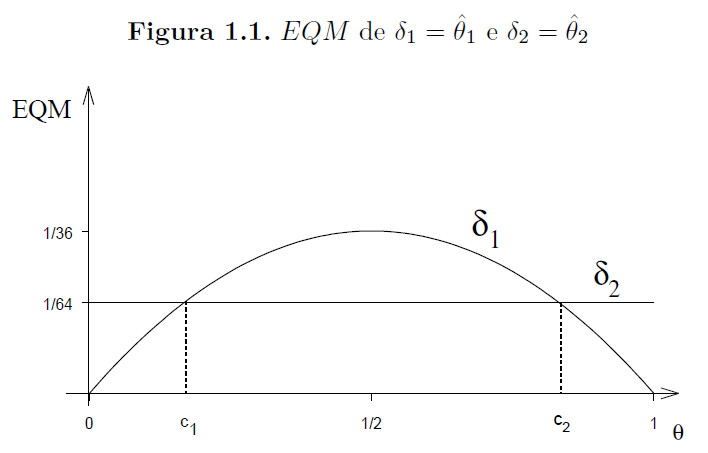
\includegraphics[scale=0.5]{figs/EQM.png}
    %\caption{Caption}
    \label{fig1}
\end{figure}
\end{block}
\end{frame}

\begin{frame}{Continuação do Exemplo 3}
\begin{block}{}
\justifying
Temos, então, que nenhum dos estimadores é melhor uniformemente, isto é, para todo $\theta$. Para $c_1 < \theta < c_2$, $EQM[\hat{\theta}_2] < EQM[\hat{\theta}_1]$, ou seja, $\hat{\theta}_2$ é melhor que $\hat{\theta}_1$. Por outro lado, para $\theta < c_1$ ou $\theta > c_2$, temos que $EQM[\hat{\theta}_1] < EQM[\hat{\theta}_2]$, ou seja, $\hat{\theta}_1$ é melhor que $\hat{\theta}_2$.
\end{block}
\end{frame}

\subsection{Estimador Não Viesado de Variância Mínima Uniformemente}
\begin{frame}{Estimador Não Viesado de Variância Mínima Uniformemente (ENVVMU)}
\begin{block}{}
\justifying
Um estimador $\hat{\theta}^{*}$ é um estimador não viesado de $\theta$ se satisfaz $E(\hat{\theta}^{*})=\theta$ e, para qualquer outro estimador $\hat{\theta},$ temos que $Var(\hat{\theta}^{*})\leq Var(\hat{\theta}),~\forall~ \theta.$ $\hat{\theta}^{*}$ é também chamado de Estimador Não Viesado de Variância Mínima Uniformemente (ENVVMU) de $\theta.$
\end{block}
\end{frame}

\begin{frame}{Eficiência Relativa de um Estimador}
\begin{block}{}
\justifying
O erro quadrático médio é uma métrica importante e pode ser usado para definir a eficiência relativa de um estimador comparado a outro:
\begin{align*}
    EFR(\hat{\theta}_{1}, \hat{\theta}_{2})=\dfrac{EQM(\hat{\theta}_{1})}{EQM(\hat{\theta}_{2})}
\end{align*}
Se $E(\hat{\theta}_1, \hat{\theta}_2) < 1$, conclui-se que $\hat{\theta}_1$ é um estimador superior a $\hat{\theta}_2$ ou vice-versa.
\end{block}
\end{frame}

\begin{frame}[allowframebreaks]
\frametitle{\bf Referências}
\printbibliography
\end{frame}


\end{document}


\subsection{Consistência}
\begin{frame}{}
\begin{block}{}
\justifying
Consistência está ligada ao conceito de convergência em probabilidade.

Sejam $X_1, \ldots, X_n$ uma amostra aleatória da distribuição da variável aleatória $X$ que depende do parâmetro $\theta$. Dizemos que o estimador $\hat{\theta} = \hat{\theta}(X_1, \ldots, X_n)$ é consistente para o parâmetro $\theta,$ se,
\begin{align*}
    \lim_{n\rightarrow \infty} P(|\hat{\theta}-\theta|>\epsilon)=0
\end{align*}
\end{block}
\end{frame}

\begin{frame}{Exemplo}
\begin{block}{}
\justifying
Sejam $X_1, \ldots, X_n$ uma amostra aleatória de tamanho $n$ da distribuição da variável aleatória $X$ com média $\theta$ e variância $\sigma^2$. Temos, usando a desigualdade de Chebyshev, que, $$P(|\Bar{X}-\theta|>\epsilon)\leq \dfrac{\sigma^{2}}{n\epsilon^{2}},$$ 
de modo que,
$$\lim_{n\rightarrow \infty} P(|\Bar{X}-\theta|>\epsilon)=0,$$
e portanto $\Bar{X}$ é consistente para $\theta$.
\end{block}
\nocite{hogg}\nocite{casella2021statistical} \nocite{bolfarine}
\end{frame}